\documentclass[a4paper,12pt]{article}
\usepackage[utf8]{inputenc}
\usepackage[spanish]{babel}
\usepackage{color}
\usepackage{parskip}
\usepackage{graphicx}
\usepackage{multirow}
\usepackage{listings}
\usepackage{vmargin}
\usepackage{datetime}
\newdate{date}{12}{10}{2017}
\graphicspath{ {imagenes/} }
\definecolor{mygreen}{rgb}{0,0.6,0}
\definecolor{lbcolor}{rgb}{0.9,0.9,0.9}
\usepackage{epstopdf}
\usepackage{float}


\setpapersize{A4}
\setmargins{2.5cm}       % margen izquierdo
{1.5cm}                        % margen superior
{16.5cm}                      % anchura del texto
{23.42cm}                    % altura del texto
{10pt}                           % altura de los encabezados
{1cm}                           % espacio entre el texto y los encabezados
{0pt}                             % altura del pie de página
{2cm}     

\lstset{
%backgroundcolor=\color{lbcolor},
    tabsize=4,    
%   rulecolor=,
    language=[GNU]C++,
        basicstyle=\tiny,
        aboveskip={1.5\baselineskip},
        columns=fixed,
        showstringspaces=false,
        extendedchars=false,
        breaklines=true,
        prebreak = \raisebox{0ex}[0ex][0ex]{\ensuremath{\hookleftarrow}},
        frame=single,
        showtabs=false,
        showspaces=false,
        showstringspaces=false,
        identifierstyle=\ttfamily,
        keywordstyle=\color[rgb]{0,0,1},
        commentstyle=\color[rgb]{0.026,0.112,0.095},
        stringstyle=\color{red},
        numberstyle=\color[rgb]{0.205, 0.142, 0.73},
%        \lstdefinestyle{C++}{language=C++,style=numbers}’.
}


\begin{document}
\title{Tarea de Laboratorio 2}
\author{
Christofer Fabián Chávez Carazas \\
\small{Universidad Nacional de San Agustín de Arequipa} \\
\small{Escuela Profesional de Ciencia de la Computación} \\
\small{Compiladores}
}
\date{\displaydate{date}}

\maketitle

El objetivo de la práctica era crear un pequeño compilador que traduzca un pseudocodigo a lenguaje c++.
El pseudocodigo es el siguiente:

\begin{lstlisting}
Inicio
variables a,b,c:entero
Leer a
Leer b
c<-a+b
Escribir c
\end{lstlisting}

El programa es el siguiente:

\begin{lstlisting}
#include <iostream>
#include <vector>
#include <cstdio>

using namespace std;

enum Errores {TIPE,ASIG,NOEXVAR,GENERROR};

class Error{
public:
	Error(int a, int b, string s){
		numLinea = a;
		error = b;
		linea = s;
	}
	int numLinea;
	int error;
	string linea;
};
	

int IDfind(vector<string> &v, string s){
	for(int i = 0; i < v.size(); i++){
		if(v[i] == s) return i;
	}
	return -1;
}

bool find(vector<string> &v, string s){
	if(IDfind(v,s) == -1) return false;
	return true;	
}

int main(int argc, char const *argv[]){
	string line = "";
	int estado = 0;
	int numLinea = 0;
	vector<string> idVariables;
	vector<string> tipoVariables;
	try{
		while(true){
			cin>>line;
			numLinea++;
			if(estado == 0 and line == "Inicio"){
				cout<<"#include <iostream>"<<endl<<"using namespace std;"<<endl<<"int main(int argc, char const *argv[]){"<<endl;
				estado = 1;
			} 
			else if(estado == 1 and line == "variables") estado = 2;
			else if(estado == 2){
				string temp = "";
				int num = 0;
				for(char c : line){
					if(c == ',' or c == ':'){
						num++;
						idVariables.push_back(temp);
						temp.clear();
					}
					else temp.push_back(c);
				}
				if(temp != "entero" and temp != "real"){
					throw(Error(numLinea,TIPE,line));
				}
				for(int i = 0; i < num; i++){
					tipoVariables.push_back(temp);
				}
				for(int i = 0; i < idVariables.size(); i++){
					string tipo = "";
					if(tipoVariables[i] == "entero") tipo = "int";
					else if(tipoVariables[i] == "real") tipo = "float";
					cout<<tipo<<" "<<idVariables[i]<<";"<<endl;
				}
				estado = 3;
			}
			else if(estado == 3){
				if(line == "Leer") estado = 4;
				else{
					string temp = "";
					string uno = "";
					string dos = "";
					string tres = "";
					int subestado = 0;
					for(char c : line){
						if(subestado == 0 and c == '<'){
							if(!find(idVariables,temp)) throw(Error(numLinea,NOEXVAR,line));
							uno = temp;
							temp.clear();
							subestado = 1;
						}
						else if(subestado == 1){
							if(c != '-'){
								throw(Error(numLinea,ASIG,line));
							}
							else{
								//temp.push_back(c);
								subestado = 2;	
							}
						}
						else if(subestado == 2 and c == '+'){
							if(!find(idVariables,temp)) throw(Error(numLinea,NOEXVAR,line));
							dos = temp;
							temp.clear();
							subestado = 3;
						}
						else temp.push_back(c);
					}
					if(!find(idVariables,temp)) throw(Error(numLinea,NOEXVAR,line));
					tres = temp;
					cout<<uno<<"="<<dos<<"+"<<tres<<";"<<endl;
					estado = 5;
				}
			}
			else if(estado == 4){
				if(!find(idVariables,line)) throw(Error(numLinea,NOEXVAR,line));
				cout<<"cin>>"<<line<<";"<<endl;
				estado = 3;
			}
			else if(estado == 5 and line == "Escribir")  estado = 6;
			else if(estado == 6){
				if(!find(idVariables,line)) throw(Error(numLinea,NOEXVAR,line));
				cout<<"cout<<"<<line<<"<<endl;"<<endl;
				estado = 7;
			}
			else if(estado == 7){
				cout<<"return 0;"<<endl<<"}"<<endl;
				break;
			}
			else throw(Error(numLinea,GENERROR,line));
		}
	}
	catch(Error e){
		fprintf(stderr,"Line %d:%s\n",e.numLinea,e.linea.c_str());
		switch(e.error){
			case TIPE:
				fprintf(stderr,"No existe el tipo\n");
				break;
			case ASIG:
				fprintf(stderr,"Error en la operacion asignacion\n");
				break;
			case NOEXVAR:
				fprintf(stderr,"No existe la variable\n");
				break;
			case GENERROR:
				fprintf(stderr,"ERROR\n");
				break;
		}
	}
	return 0;
}
\end{lstlisting}

El compilador va generando el código intermedio mientras va leyendo el pseudocodigo. El programa cuenta con un contador de líneas para un mejor manejo de los errores. Los identificadores son guardados en el vector \textit{idVariables}, mientras que
sus respectivos tipos son guardados en el vector \textit{tipoVariables}. El compilador reconoce variables de tipo entero y real, y cada vez que se necesita, realiza una
búsqueda en el vector \textit{idVariables} para verificar que el identificador no esté repetido o que sí exista.

\textbf{Resultados:}

\begin{itemize}
 \item \textbf{Con el pseudocodigo sin alterar:}


\begin{figure}[H]
 \centering
 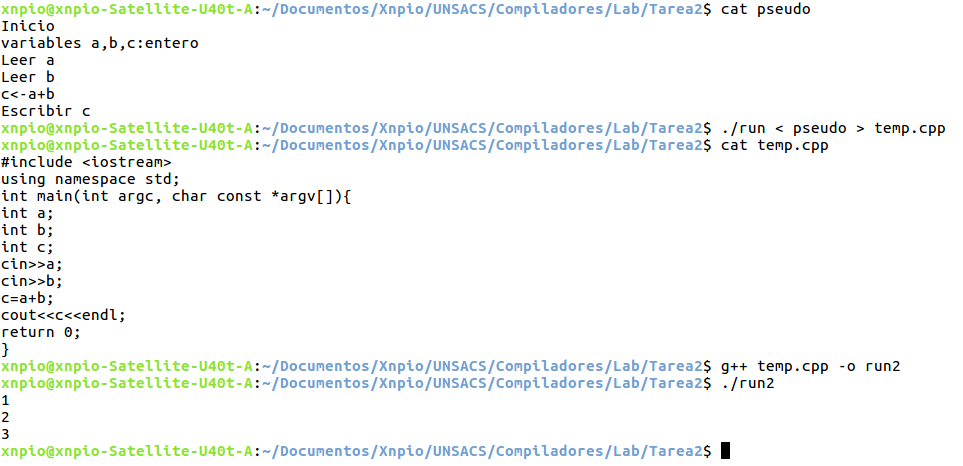
\includegraphics[scale = 0.5]{1.png}
\end{figure}

 \item \textbf{Cambiando el tipo entero por real:}
 
\begin{figure}[H]
 \centering
 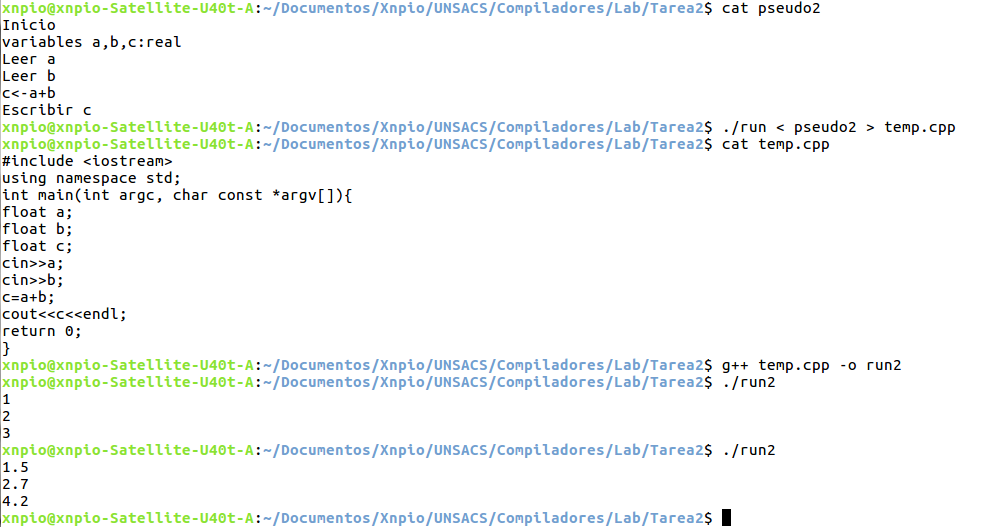
\includegraphics[scale = 0.5]{2.png}
\end{figure}

 \item \textbf{Leyendo una variable que no ha sido definida:}
 
\begin{figure}[H]
 \centering
 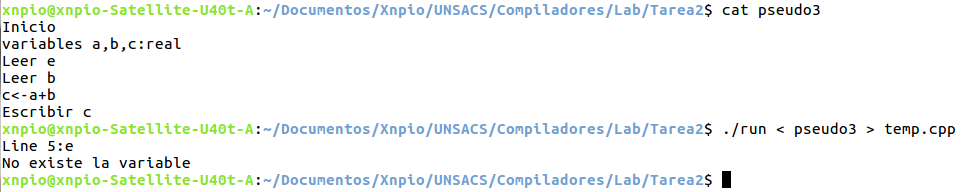
\includegraphics[scale = 0.5]{3.png}
\end{figure}

 \item \textbf{Poniendo un tipo que no es reconocido:}
 
\begin{figure}[H]
 \centering
 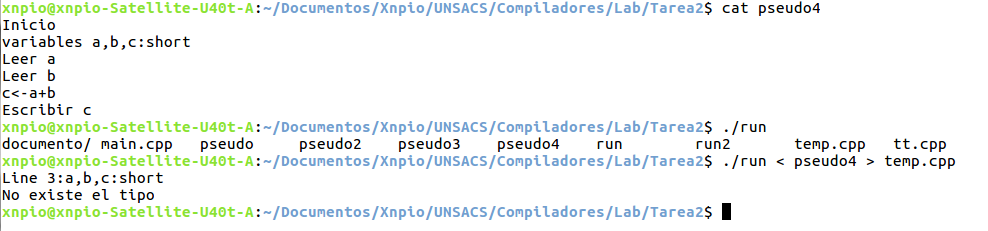
\includegraphics[scale = 0.5]{4.png}
\end{figure}


\end{itemize}
\end{document}

